\begin{frame}{Transfer Learning}
  \begin{figure}
    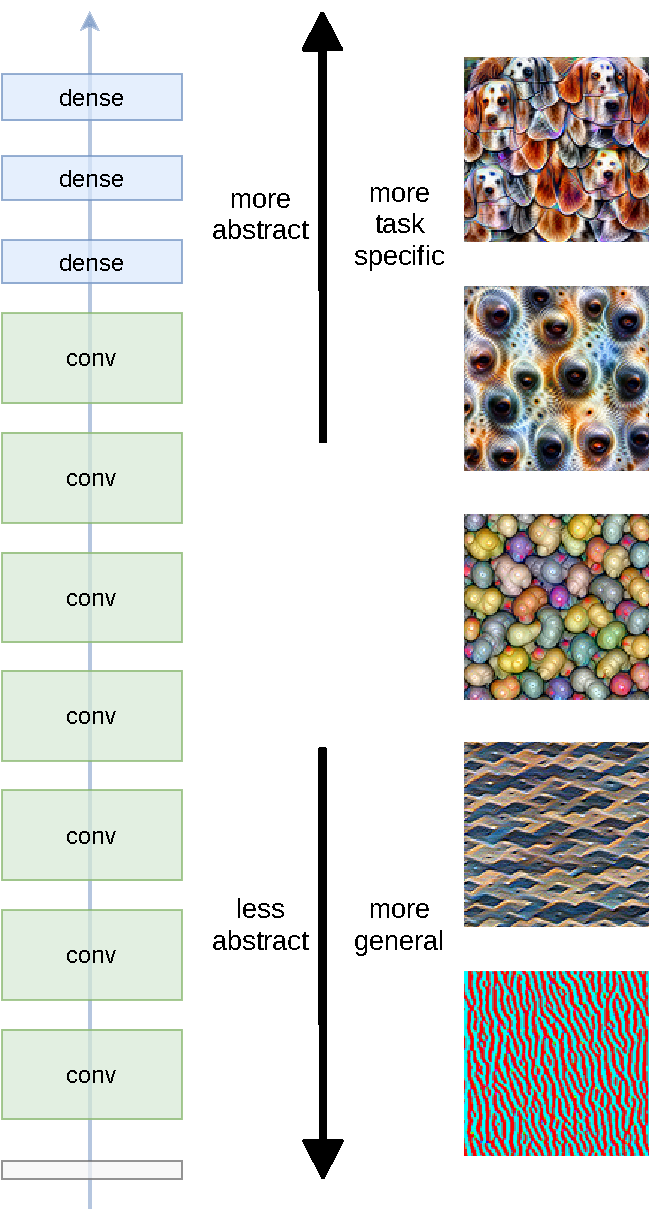
\includegraphics[width=0.3\textwidth]{tl_00}
  \end{figure}

  \note{
    \begin{itemize}
      \item Deep learning needs big data!
      \item But what if we use the more general abilities a network learned for another task?
      \item Images from Feature Visualization, Olah et al, https://distill.pub/2017/feature-visualization/
    \end{itemize}
  }
\end{frame}


\begin{frame}{Transfer Learning}
  \begin{figure}
    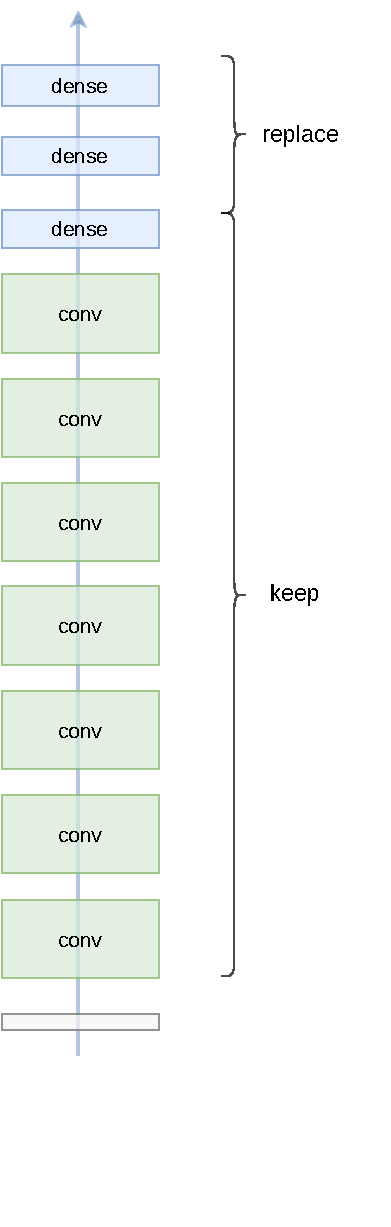
\includegraphics[width=0.2\textwidth]{tl_01}
  \end{figure}
  \note{
    \begin{itemize}
      \item We can transfer knowledge by replacing the specialized layers with randomly initialized layers and only train those!
    \end{itemize}
  }
\end{frame}


\begin{frame}{Transfer Learning: fine tuning}
  \begin{columns}
    \begin{column}{0.2\textwidth}
      \begin{figure}
        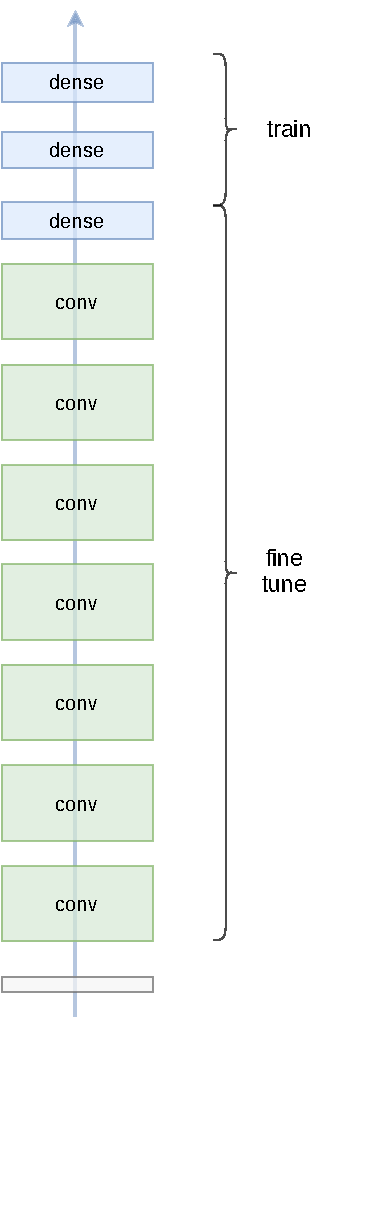
\includegraphics[width=0.8\textwidth]{tl_02}
      \end{figure}
    \end{column}
    \begin{column}{0.8\textwidth}
      \begin{itemize}
        \item 1. Train the randomly initialized layers to convergence.
        \item 2. Unfreeze the some of the upper layers and continue training.
      \end{itemize}
    \end{column}
  \end{columns}
  \note{
    \begin{itemize}
      \item Randomly initialized layers generate high gradients, which would destroy what was learned in the layers below.
      \item Fine tune with very small learning rate ($\approx .1\times$ original lr)
    \end{itemize}
  }
\end{frame}


\begin{frame}{Transfer Learning}
  \begin{columns}
    \begin{column}{0.2\textwidth}
      \begin{figure}
        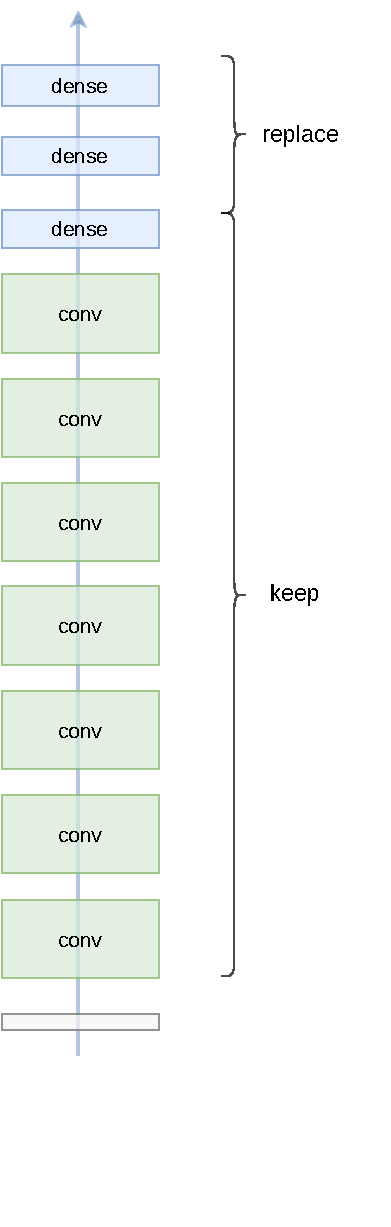
\includegraphics[width=0.8\textwidth]{tl_01}
      \end{figure}
    \end{column}
    \begin{column}{0.8\textwidth}
      \begin{itemize}
        \item The more data we have for the target domain \\
              $\rightarrow$ the more layers we can replace.\\
              $\rightarrow$ the more layers we can fine tune.\\
        \item The higher the distance between original and target task \\
              $\rightarrow$ the more layers we may want to replace.\\
              $\rightarrow$ the more layers we need to fine tune.\\
      \end{itemize}
    \end{column}
  \end{columns}

  \note{
    \begin{itemize}
      \item Give it a try, it works surprisingly well.
      \item Transfer learning has become the default initialization.\\
            (In many frameworks, it's just an argument in a function call to initialize with weights trained on ImageNet.)
      \item Recent results show, that it is not always necessary.\\
            (Rethinking ImageNet Pre-training, He et al, ICCV 2019)
    \end{itemize}
  }
\end{frame}
